% -*- coding: UTF-8 -*-
% vim: autoindent expandtab tabstop=4 sw=4 sts=4 filetype=tex
% chktex-file 27 - disable warning about missing include files

\section{Beleuchtungsmodelle}
\label{sec:illumination_models}

Sofern nicht anders vermerkt, basiert der folgende Abschnitt auf~\cite{whitted_improved_1980}[S. 343] sowie auf~\cite{hughes_computer_2013}.

Beleuchtungsmodelle beschreiben, wieviel Licht von einem sichtbaren Punkt einer Oberfläche zum Betrachter emitiert wird. In der Regel wird das Licht als Funktion in Abhängigkeit folgender Faktoren beschrieben:
\begin{itemize}
    \item Richtung der Lichtquelle \item Lichstärke
    \item Position des Betrachters
    \item Orientierung der Oberfläche
    \item Oberflächenbeschaffenheit
    \item Globale Umgebung
\end{itemize}

Es wird dabei zwischen lokalen und globalen Belechtungsmodellen unterschieden.

\subsection{Lokale Beleuchtungsmodelle}
\label{subsec:local_illumination_models}

Lokale Beleuchtungsmodelle aggregieren Daten von benachbarten, eben lokalen,
Oberflächen. Diese Modelle sind in deren Umfang allerdings limitiert, da sie
normalerweise nur Lichtquellen sowie die Orientierung einer Oberfläche
einbeziehen. Sie ignorieren dabei aber die globale Umgebung, in welcher sich
eine Oberfläche befindet.  Dies ist dadurch bedingt, dass die traditionell
verwendeten Algorithmen zur Berechnung der Sichtbarkeit von Oberflächen, über
keine globalen Daten verfügen. Das bekannteste lokale Beleuchtungsmodell ist
das \textbf{Phong}-Beleuchtungsmodell, welches 1975 von Phong Bui-Tong
entwickelt wurde. Es beschreibt nicht-perfekte Reflektoren wie zum Beispiel einen
Apfel~\cite{foley_computer_1996}[Kapitel 16, Seite 729].

\begin{figure}[H]
    \centering
    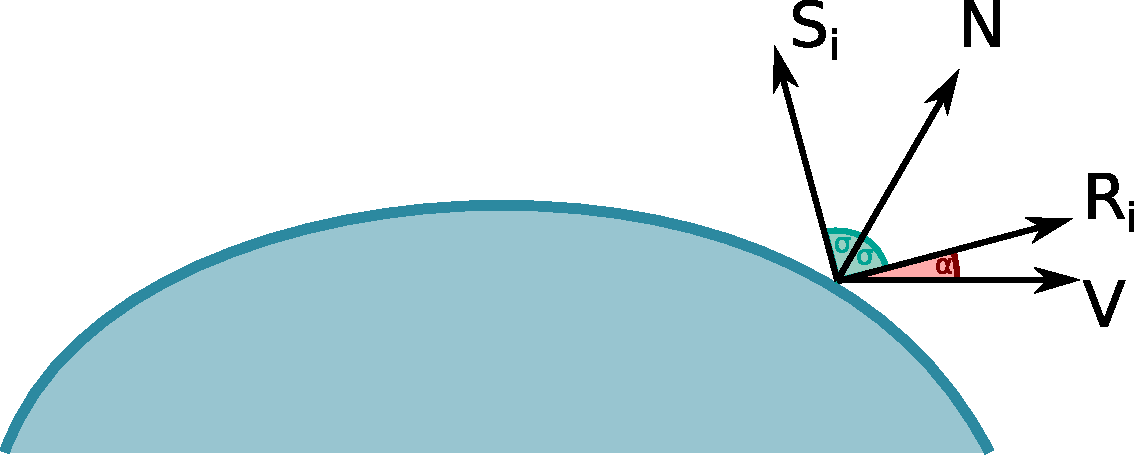
\includegraphics[width=0.6\textwidth]{img/phong_illumination_model.pdf}
    \caption{Illustration des Phong-Beleuchtungsmodelles\protect\footnotemark}\label{fig:phong_illustration}
\end{figure}
\footnotetext{Eigene Darstellung mittels Geogebra, angelehnt an~\cite{foley_computer_1996}[Kapitel 16, Seite 731, Abbildung 16.12]}

Es beschreibt die reflektierte (Licht-) Intensität als Zusammensetzung aus der ambienten, der diffusen und der ideal spiegelnden Reflexion einer Oberfläche:

\begin{gather}
    I = I_{\text{ambient}} + I_{\text{diffuse}} + I_{\text{specular}} + I_{\text{emissive}}
\end{gather}

oder mathematisch ausgedrückt:

\begin{gather}
    I(\vv{V}) = k_{a} \cdot L_{a} +
                k_{d} \displaystyle\sum_{i=0}^{n - 1} L_{i} \cdot (\vv{S_{i}} \cdot \vv{N}) +
                k_{s} \displaystyle\sum_{i=0}^{n - 1} L_{i} \cdot {(\vv{R_{i}} \cdot \vv{V})}^{k_{e}}
\end{gather}

wobei gilt:

\begin{itemize}
    \item $I(\vv{V})$:              Die reflektierte (Licht-) Intensität in Richtung des Vektors $\vv{V}$
    \item $n$:                      Anzahl Lichtquellen
    \item $k_{a} \cdot L_{a}$:      Ambiente Komponente des
                                    Beleuchtungsmodelles. Mittels diesem Faktor
                                    wird versucht allem indirekten Licht der
                                    Szene gerecht zu werden. Bei $k_{a}$
                                    handelt es sich um eine Konstante, welche
                                    den ambienten Lichtanteil $L_{a}$ skaliert
    \item $k_{d}$:                  Konstante für die diffuse Komponente des
                                    reflektierten Lichtes, basierend auf der
                                    Wellenlänge bzw. Frequenz
    \item $\vv{S_{i}}$:             Richtung, in welcher das Licht der $i$-ten
                                    Lichtquelle ankommt, normalisierter
                                    Einheitsvektor
    \item $\vv{N}$:                 Einheitsnormale der Oberfläche
    \item $k_{s}$:                  Koeffizient der spiegelenden Komponente,
                                    basierend auf der Wellenlänge bzw. Frequenz
    \item $\vv{R_{i}}$:             Richtung, in welcher das Licht der $i$-ten
                                    Lichtquelle reflektiert wird,
                                    normalisierter Einheitsvektor
    \item $\vv{V}$:                 Blickrichtung des Betrachters bzw.\ der
                                    Kamera
    \item $k_{e}$:                  Exponent, welcher von der Rauheit bzw.
                                    Reflektion der Oberfläche abhängt
    \item $L_{i}$                   Licht- bzw.\ Farbintnsität der $i$-ten
                                    Lichtquelle
\end{itemize}

Meist wird der emissive Term bewusst weggelassen, da dieser meist eher für
Spezialeffekte statt für die Beleuchtung ``normaler'' Objekte benutzt wird.

Der reflektive Vektor $R_{i}$ ist gegeben durch

\begin{gather}
    R_{i} = S_{i} + 2(S_{i} \cdot N)N
\end{gather}

Damit die Energieerhaltung gewährleistet ist, muss weiter $k_{d} + k_{s} < 1$
gelten. Der Winkel zwischen $\vv{R}$ und $\vv{V}$ wird mittels $\cos{\alpha}$
ermittelt.


\subsection{Globale Beleuchtungsmodelle}
\label{subsec:global_illumination_models}

Sofern nicht anders vermerkt, basiert der folgende Abschnitt auf~\cite{foley_computer_1996}[S. 775ff]

Globale Beleuchtungsmodelle beschreiben die reflektierte (Licht-) Intensität
eines Punktes aufgrund direkter Lichteinstrahlung durch Lichtquellen sowie
durch alles Licht, welches diesen Punkt nach Reflektion von bzw. Durchdringen
der eigenen oder anderer Oberflächen erreicht.

Bei globalen Beleuchtungsmodellen unterscheidet man zwischen
blickwinkelabhängigen Algorithmen, wie etwa Ray Tracing, und zwischen
blickwinkelunabhängigen Algorithmen, wie etwa Photon Mapping.

Blickwinkelabhängige Algorithmen verwenden eine Diskretisierung der sichtbaren
Fläche bzw. Bildfläche um zu entscheiden, an welchen Punkten, in Blickrichtung
des Betrachters, die Beleuchtungsberechnung durchgeführt werden soll.
Blickwinkelunabhängige Algorithmen hingegen diskretisieren und verarbeiten die
Umgebung um genügend Informationen für die Beleuchtungsberechnung zu haben.
Dies erlaubt ihnen die Beleuchtungsberechnung an einem beliebigen Punkt aus
einer beliebigen Blickrichtung.

Beide Arten von Algorithmen haben jedoch Vor- und Nachteile. So sind
blickwinkelabhängige Algorithmen gut geeignet um Spiegelungen, basierend auf
der Blickrichtung des Betrachtes, zu berechnen, eignen sich aber weniger um
gleichbleibende diffuse Anteile über weiter Flächen eines Bildes zu berechnen.
Bei blickwinkelabhängigen Algorithmen verhält es sich genau umgekehrt.

\subsubsection{Renderinggleichung}
\label{ssubsec:rendering_equation}

Die unter~\ref{subsec:global_illumination_models} genannten Verfahren versuchen
auszudrücken, wie sich Licht von einem Punkt im Raum zu einem anderen bewegt.
Dabei beschreiben sie die Intensität des Lichtes, ausgehend vom ersten Punkt
zum zweiten Punkt. Zusätzlich wird die Intensität des Lichtes, ausgehend von
allen anderen Punkten, welche den ersten Punkt erreichen, und zum zweiten Punkt
emitiert werden, beschrieben.

James (Jim) Kajiya stellte 1986 die so genannte Renderinggleichung auf, welche
genau dieses Verhalten beschreibt~\cite{kajiya_rendering_1986}
und~\cite{foley_computer_1996}:
\begin{equation}
    I(x, x') = g(x, x')[\varepsilon(x, x') + \int\limits_{S}\rho(x, x', x'')I(x', x'')dx'']
\end{equation}
wobei gilt:

\begin{itemize}
    \item $x, x' \text{und } x''$: Punkte in der Umgebung
    \item $ I(x, x')$:            Lichtintensität von Punkt $x'$ nach Punkt $x$
    \item $ g(x, x')$:            Ein auf die Geometrie bezogener Term\\
                                  \hspace*{4mm} $0$:     \hspace*{6mm} $x$ und $x'$ verdecken sich\\
                                  \hspace*{4mm} $1/r^2$: \hspace*{1mm} $x$ und $x'$ sehen sich, wobei $r$ die Distanz zwischen $x$ und $x'$ ist
    \item $\epsilon(x, x')$:      Intensität des Lichtes, welches von $x'$ nach $x$ emitiert wird
    \item $\rho(x, x', x'')$:     Intensität des Lichtes, welches von $x''$
                                  durch die Oberfläche bei $x'$ nach $x$
                                  gestreut wird
    \item $\int\limits_{S}$:      Integral über die Vereinigung aller Flächen,
                                  daher $ S = \bigcup{S_{i}} $\\
                                      Dies bedeutet, dass die Punkte $x$, $x'$
                                      und $x''$ über alle Flächen aller Objekte
                                      der Szene ``streifen''.  Wobei es sich
                                      bei $S_{0}$ um eine zusätzliche Fläche
                                      handelt, welche als Hintergrund verwendet
                                      wird.  $S_{0}$ ist dabei eine Hemisphäre,
                                      welche die gesamte Szene umspannt.
\end{itemize}

\section{Ray Casting und Ray Tracing}
\label{sec:ray_casting_tracing}

Sofern nicht anders vermerkt, basiert der folgende Abschnitt
auf~\cite{hughes_computer_2013}[Kapitel 15, S. 387ff].

Um ein Bild möglichst realistisch darzustellen muss berechnet werden, wieviel
Licht zu jedem Pixel der sichtbaren Bildfläche (also dem Betrachter)
transportiert wird. Da Photonen die Energie des Lichtes transportieren, muss
man also das physikalische Verhalten dieser simulieren.

Es ist allerdings nicht möglich \textit{alle} Photonen zu simulieren, da
der Aufwand schlicht zu gross wäre. Daher macht es Sinn nur einige
Photonen (exemplarisch) zu betrachten und dann eine Abschätzung des
gesamten Lichtes vorzunehmen.

Jede Lichtquelle emitiert Photonen (als Welle und als Teilchen) in alle
Richtungen. Man modeliert diese als Partikel, welche anhand
Lichtstrahlen (\textit{light rays}) auf Objekte einer
Szene treffen.

Jedes Photon hat dabei eine spezifische Wellenlänge ($\lambda{}$) welche
die Farbe definiert, sowie eine Energie (Frequenz $f$) welche die
Farbintensität des Photons definiert.

Trifft ein Photon auf ein Objekt, wird ein Teil der Energie absorbiert,
ein Teil reflektiert und ein Teil durchdringt das Objekt (Transmission).
Photonen treffen solange auf Objekte bis deren gesamte Energie
absorbiert, sie die Szene verlassen oder sie auf die sichtbare
Bildfĺäche treffen und somit zum eigentlichen Bild beitragen.

Bei Ray Casting bzw. Ray Tracing handelt es sich um eine relativ
einfache Art um globale Beleuchtungsmodelle zu implementieren.

Die einfachste Art Lichtstrahlen zu modellieren ist das so
genannte~\textit{Ray Casting}.


\subsection{Ray Casting}
\label{subsec:ray_casting}

\todo[inline]{Expand this section. Add formulas as well as examples.}
\todo[inline]{Punkte mehr ausführen; Integration zeigen mit Diskretition; auch Berechnungen}

Bei \textbf{Ray Casting} handelt es sich grundsätzlich um eine Strategie zur
Simulation, wieviel Licht anhand eines (Licht-) Strahles zu der sichtbaren
Bildfläche (also dem Betrachter) transportiert wird.

Das Verfahren wurde erstmals 1968 in~\cite{appel_techniques_1968} vorgeschlagen
und auch 1968 von der Matthematical Applications Group Inc.\
in~\cite{arlington_mathematical_applications_group_inc_afips_1968} erfolgreich umgesetzt.

Es wird ein ``Projektionszentrum'' (das Auge eines Betrachters) sowie
eine Region einer beliebigen Bildfläche gewählt. Dabei kann die Region
als gerasterte Fläche angenommen werden. Jedes Raster entspricht den
Bildpunkten (Pixeln) der gewünschten Auflösung.  Daher, je feiner die
Rasterung, desto höher die Auflösung.

Für jeden Bildpunkt der gewählten Region wird ein Strahl
generiert, welcher dann vom Projektionszentrum durch das Zentrum des
Bildpunktes auf die Szene ``geworfen'' wird. 

Es wird dann das Objekt gesucht, welches den nähesten Schnittpunkt mit
dem Strahl bildet. Für jede Lichtquelle der Szene wird geprüft, ob die
Lichtquelle vom Schnittpunkt aus sichtbar ist. Ist dies der Fall, wird
schliesslich die Farbe und die Farbintensität an diesem Schnittpunkt
anhand eines Beleuchtungsmodelles (z.\ B.\ dem Phong-Beleuchtungsmodell)
berechnet. Ansonsten befindet sich der Punkt im Schatten, wird also
nicht beleuchtet.

Um den Schnittpunkt eines Lichtstrahles mit einem Objekt zu berechnen
wird grundsätzlich die mathematische Gleichung des Lichtstrahles in die
des Objektes eingesetzt. Existiert eine reelle Lösung, so schneidet der
Lichtstrahl das Objekt am nähesten Punkt zwischen dem Schnittpunkt und
der Oberflächennormale des Objektes.

~\citeauthor{glassner_introduction_1989} beschreibt mehrere Methoden zur
Prüfung von Schnittpunkten, hier sei beispielhalber nur die Intersektion
mit einer Kugel sowie mit einem Dreieck genannt.

Um den Schnittpunkt bzw.\ die Schnittpunkte eines Lichtstrahles mit
einer Kugel zu erhalten, wird die Gleichung des Lichtstrahles:

\begin{gather}
    r(t) = r_{0} + t \cdot r_{d}
\end{gather}

in die implizite Gleichung einer Kugel:

\begin{gather}
    \|\bm{x} - c\|^{2} - r^{2} = 0
\end{gather}

eingesetzt:

\begin{align}
    \|r(t) - c\|^{2} - r^{2} &= 0 \\
    \|r_{0} + t \cdot r_{d} - c\|^{2} - r^{2} &= 0
\end{align}

Das Auflösen dieses Gleichungssystemes ergibt folgende Fälle:
\begin{itemize}
    \item{Zwei Lösungen}: Der Strahl geht durch die Kugel hindurch.
    \item{Eine Lösungen}: Der Strahl streift die Kugel an einem Punkt
        als Tangente.
    \item{Imaginäre Lösung}: Der Strahl verfehlt die Kugel komplett.
\end{itemize}

Um den Schnittpunkt eines Lichtstrahles mit einem Dreieck zu erhalten,
wird die Gleichung des Lichtstrahles:

\begin{gather}
    r(t) = r_{0} + t \cdot r_{d}
\end{gather}

als Lösung der Gleichung eines Dreiecks mit baryzentrischen Koordinaten:

\begin{gather}
    x(\beta, \gamma) = v_{1} + \beta(v_{2} - v_{1}) + \gamma(v_{3} - v_{1})
\end{gather}

verwendet:

\begin{align}
    r_{0} + t \cdot r_{d} &= v_{1} + \beta(v_{2} - v_{1}) + \gamma(v_{3} - v_{1})
\end{align}

Der Lichtstrahl schneidet das Dreieck genau dann, wenn gilt $\beta +
\gamma \le 1$, $\beta \ge 0$ und $\gamma \ge 0$.

Ein möglicher Algorithmus, wie Ray Tracing umgesetzt werden kann, findet
sich in~\ref{fig:ray_casting:high_level}.

\begin{lstlisting}[language=Python,caption={Eine abstrakte Umsetzung des Ray
        Castings\protect\footnotemark.},label={fig:ray_casting:high_level},captionpos=b,emph={ray_cast}]
def ray_cast():
    # "pixels" is a list of all pixels of the image plane
    for pixel in pixels:
        # Save all intersections for given pixel
        intersections = []

        # Returns the ray passing through the given
        # pixel from the eye
        ray = ray_at_pixel(pixel)

        # "scene_triangles" is a list of all triangles
        # coming from meshes contained in the scene to render
        for triangle in scene_triangles:
            p   = intersect(ray, triangle)
            sum = 0

            for light in incoming_lights_at_p:
                sum = sum + l.value
            end

            if is_smallest_intersection(p, intersections):
                pixel = sum
            intersections.append(p)
\end{lstlisting}
\footnotetext{Algorithmus in Pseudocode gemäss~\cite{hughes_computer_2013}[Kapitel 15, Seite 391, Auflistung 15.2]}

\subsection{Ray Tracing}
\label{subsec:ray_tracing}

Sofern nicht anders vermerkt, basiert der folgende Abschnitt
auf~\cite{glassner_introduction_1989}[S. 1 bis 77].

Bei dem heute als Ray Tracing bekannten Verfahren, handelt es sich um
eine verbesserte Version des unter~\ref{subsec:ray_casting} genannten
Ray Casting Verfahrens. Dieses wurde im Juni 1980
durch~\citeauthor{whitted_improved_1980} verbessert.

Grundsätzlich ist die Idee, dass jeder Bildpunkt der gewählten Region
Licht aus nur einer Richtung erhält --- derer der Lichtstrahlen
(\textit{light rays}), welche durch die gewählte Region und die
sichtbare Bildfläche gehen. Somit trägt jedes Photon, welches aus dieser
Richtung kommt, zum Farbwert bzw.\ der Farbintensität eines Bildpunktes
bei.

Die Lichtstrahlen werden in dieser Richtung verfolgt, um festzustellen
wie das Licht ``erzeugt'' wird:
\begin{itemize}
    \item{Der Lichtstrahl trifft auf nichts} --- die Strahlenverfolgung
        wird beendet, der Bildpunkt wird mit der Farbe des Hintergrundes
        eingefärbt.
    \item{Der Lichtstrahl trifft auf eine Lichtquelle} --- die
        Strahlenverfolgung wird beendet, der Bildpunkt wird mit der
        Farbe und Intensität der Lichtquelle eingefärbt.
    \item{Der Lichtstrahl trifft auf eine Oberfläche} --- der Prozess
        wird von diesem Punkt aus neu gestartet um festzustellen, wie
        das Licht dort ``erzeugt'' wurde.
\end{itemize}

Wie der letzte Punkt zeigt, handelt es sich also um ein rekurisves Verfahren
und wird daher teilweise auch rekurisves Ray Tracing genannt.

\citeauthor{glassner_introduction_1989} unterscheidet analog zu den
genannten Fällen zwischen folgenden Typen von Strahlen:
\begin{itemize}
    \item{\textit{Pixel- oder Augen-Strahlen}:} Strahlen, welche das Licht von
        einer Lichtquelle durch einen Bildpunkt direkt zu der sichtbaren
        Bildfläche (also dem Betrachter) transportieren.

        $R(t) = E + t(P - E)$ wobei gilt $t \in [1, \infty]$
        \todo[inline]{E:\ Eye, P:\ Pixel}

    \item{\textit{Licht- oder Schatten-Strahlen}:} Strahlen, welche das Licht von
        einer Lichtquelle direkt zu einer Oberfläche eines Objektes
        transportieren.

        $R(t) = S + t(L - S)$ wobei gilt $t \in [\epsilon, 1]$
        \todo[inline]{S:\ Shadow spot, L:\ Lightsrc}

    \item{\textit{Reflektions-Strahlen}:} Strahlen, welche das an einem
        Objekt gespiegelte Licht transportieren.

        $R(t) = S + tB$ wobei gilt $t \in [\epsilon, \infty]$
        \todo[inline]{S:\ Shadow spot, B:?}

    \item{\textit{Transparenz-Strahlen}:} Strahlen, welche Licht
        transportieren, dass durch ein Objekt hindurch geht.
\end{itemize}~\cite{glassner_introduction_1989}[S. 10]

Zur Berechnung des emitierten Lichtes an einem gewissen Punkt eines Objektes
wird in einem ersten Schritt die Lichtintensität dieses Punktes
bestimmt.

In einem weiteren Schritt wird berechnet, wie die Oberfläche an diesem
Punkt Licht in eine spezifische Richtung weitergibt.  Dies geschieht
durch die Lichtintensität des Punktes sowie dessen physikalischen
Eigenschaften. 

Die oben genannten Strahlenarten \textit{Schatten, Reflektion und
    Transparenz} beschreiben die Prinzipien, wie Licht an einem Punkt
ankommt und sich von diesem entfernt.

Die Eigenschaften von Licht, welches direkt von einer Lichtquelle kommt
und dann weiter emitiert bzw.\ propagiert wird, werden durch
die~\textit{Schatten-Strahlen} bestimmt. Bei jedem Schnittpunkt eines
Lichtstrahles mit einem Objekt wird ein Schatten-Strahl in Richtung jeder
Lichtquelle der Szene ``geworfen''. Trifft der Schatten-Strahl die
Lichtquelle, wird das Licht zur Berechnung der Farbe und Lichtintensität
genutzt. Trifft der Schatten-Strahl keine Lichtquelle, so wird das Licht
nicht berücksichtigt. Schatten-Strahlen generieren keine weiteren
Lichtstrahlen.

Trifft ein Lichtstrahl auf eine Oberfläche wird dieses zu gewissen
Teilen~\textit{absorbiert}, \textit{reflektiert} und \textit{gebrochen}.
Die jeweiligen Anteile hängen dabei vom Medium der Oberfläche bzw.\ des
Objektes, der Frequenz des Lichtes sowie dem Winkel zwischen dem
Eingangswinkel des Lichtstrahles und der Oberflächennormale ab. Licht
kann je nach Medium auch gestreut werden.

Die Eigenschaften von Licht, welches auf ein Objekt trifft und dann an
diesem gespiegelt wird, werden durch die~\textit{Reflektions-Strahlen}
bestimmt. Handelt es sich dabei um eine perfekte spekuläre Reflektion,
so wird die eingehende Energie, ausgehend nur in eine Richtung
reflektiert.
\todo[inline]{Add image and formula for perfect specular reflection and
    perfect diffuse reflection}

Und schliesslich werden die Eigenschaften von Licht, welches durch ein
Objekt hindurch geht und vielleicht von diesem gebrochen wird, durch
die~\textit{Transparenz-Strahlen} beschrieben. Tritt Licht in ein neues
Medium ein (z.B.\ von Luft in Wasser), so wird das Licht gebrochen.
Dabei wird die Bahn des Lichtstrahles nach innen hin abgelenkt, wenn das
Licht in ein Medium mit höherer Dichte eintritt.
\todo[inline]{Add image and formula for refraction (perfect specular
    transmission), total internal reflection and transmission}

Ein möglicher Algorithmus, wie solch ein Verfahren umgesetzt werden kann,
findet sich in~\ref{fig:ray_tracing:high_level}.

\begin{lstlisting}[language=Python,caption={Eine abstrakte Umsetzung des
        Ray Tracings \protect\footnotemark.},
    label={fig:ray_tracing:high_level},captionpos=b,emph={ray_trace}]
def ray_trace(current_point, direction):
"""Traces light rays from current point in space in given direction.

:param current_point: current point in space
:type  current_point: three dimensional point object
:param direction:     the direction to trace
:type  direction:     three dimensional vector

:return:              the color for the given point
:rtype:               float
"""

    # Set color to currently set background color
    color = self.background_color

    # "pixels" is a list of all pixels of the image plane
    for pixel in pixels:

        # Returns the ray passing through the given
        # pixel from the eye
        ray = ray_at_pixel(pixel)

        # object_list is a list containing all the meshes contained in
        # the scene to render
        for object in object_list:
            p = intersect(ray, object)

            if object.is_reflective:
                reflection_vector = reflect(direction, object)
                reflected_color   = ray_trace(p, reflection_vector)
                color = color + object.coeff * reflected_color

            if object.is_refractive:
                refracted_vector = refract(direction, object)
                refracted_color  = ray_trace(p, refracted_vector)
                color = color + object.coeff * refracted_color

            for light in incoming_lights_at(p):
                if not is_shadow_ray(p, light.position):
                    color = color + calc_lighting(p, direction, light, object)
            end
        end
    end

    return color
end
\end{lstlisting}
\footnotetext{Algorithmus in Pseudocode
    gemäss~\cite{glassner_introduction_1989}[Seite 283]}
